\section{Incremental User Discovery} \label{sec:Pipeline}

The content processing pipeline operates iteratively on a set of contexts, one at the time, that is dynamically updated at the end of each iteration, starting from an initial set of seed contexts.
The user discovery process is therefore potentially open-ended, as long as new contexts can be discovered, as explained below.
Each iteration takes a context $C$  as input, and generates a list of users who participate in $C$, along with the complete set of their features and metrics as described above. 
The users profiles are added to a database, where entries for repeat users are updated according to a user-defined function. 
The final step in the iteration involves semi-automatically discovering new contexts, thus making further iterations possible.
%
The pipeline structure and data flow are illustrated in Fig. ~\ref{fig:twitterframework}.

\begin{figure*}
	\centering
	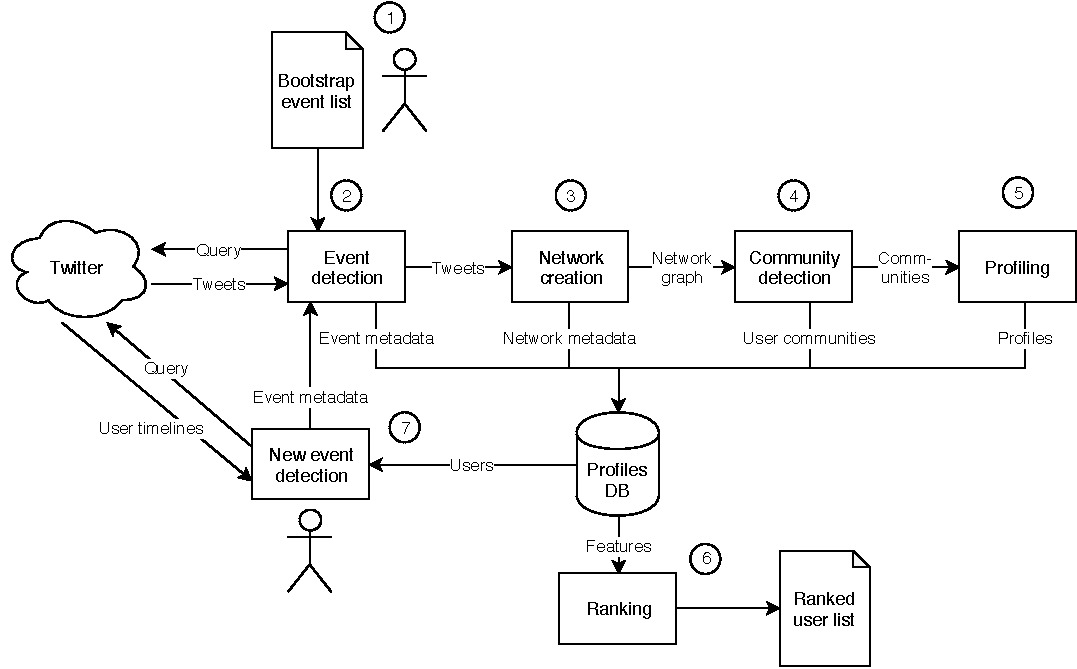
\includegraphics[width=0.7\linewidth]{figures/TwitterFramework}
	\caption{\comment{Schematic diagram of the user discovery framework }{this is a placeholder -- to be redrawn -PM }}
	\label{fig:twitterframework}
\end{figure*}

\subsection{Harvesting Content and Creating Context networks} \label{sec:harvesting}

Firstly, all Twitter posts $P(C)$ that satisfy the criteria set in $C$ are retrieved, using either the Search or the Streaming Twitter APIs.\footnote{Repeat queries and multiple accounts are used to get around the well-known Twitter API limitations for retrieving tweets.}
%
Secondly, the context network $G_C$ is generated as defined in Sec.~\ref{sec:contexts}. To recall, this is a directed network representing retweet and/or mention interactions between pairs of users in $C$. 
The size of the network is largely determined by the nature of the context, and  ranges between 140 and 400 users (avg 254, see Table~\ref{tab:networks}).

\subsection{Community detection} \label{sec:communities}

Next, the context network graph $G_C$  is partitioned into communities of users.
The goal of this partitioning is to further narrow the scope for the topology-sensitive metrics, namely FollowerRank (\ref{eq:FR}) and in-degree centrality (\ref{eq:IDC}), 
and thus to enable weak-signal users to emerge relative to other more globally dominant users.
%
Many different approaches have been proposed to discover virtual communities in social networks. 
We have chosen \demon~\cite{Coscia:2012:DLD:2339530.2339630} because it allows communities to overlap to a degree that is tunable, making it an ideal feature to identify users who may be active in more than one community within the same context, i.e., a social event or a campaign.

\demon identifies communities that a person belongs to with \textit{ego networks}, which consists of an individual, called the ego, and all the persons the ego has a social relationship with. 
As each ego network considers a node and its neighbours only, it provides a local method for discovering user affiliations, thus more akin to a social context.
%
It has been suggested~\cite{Arnaboldi2013} that ego networks are a useful model not only to describe social relationships amongst people offline, but also the structure of their online connections. 
Recognising that any individual may have different types of social relationships with different people (i.e., family, friends, colleagues, etc.),  \demon  naturally allows for an individual to participate in multiple communities. 

The locality principle of ego networks translates into an efficient algorithm for discovering overlapping communities in a social graph. 
Specifically, \demon operates on one node $v$ at a time in our context network $G_C$.

It applies a \textit{label propagation} algorithm to each neighbour $v'$ of $v$, as follows. First, a new label $l$, which identifies a new community, is tentatively assigned to $v'$. 
	Then, with probability $\alpha$ $v'$ changes its label to that of the majority of its own neighbours. 
	At this point, each of $v$'s neighbours has a label, which is either new or that of the majority of its own neighbours (except $v$ itself).
	$v$ is then assigned majority labels amongst those of its neighbours. 
	This determines $v$'s community. 
	When more than one label has the same count, $v$ is assigned to all of those communities.
%
As a final step, communities that overlap by more than some percentage $\epsilon $ are merged.

Note that users who do not belong to any community are discarded from the whole process.
Once communities are identified, we calculate  in-degree centrality (\ref{eq:IDC}) for each node locally, \textit{relative to their own community}.

\comment{In our evaluation we have experimented with varying values for parameters $\alpha$ an $\epsilon$...}{do we plan to say anything on how to tune them?}

\anote{what happens when nodes belong to more than one community?}

\subsection{Computing user features and ranking  \anote{PM to fix wording}}  \label{sec:features}

The next step in the process involves retrieving the core features and then the user relevance metrics as defined in Sec. ~\ref{sec:metrics}, for each user in each of the communities.
%
As this involves querying the Twitter API for many user profiles, this step hits the limitations imposed by Twitter \anote{be specific}.
To get around this problem, we have implemented a dedicated component to \textit{scrape} user information directly from their profile Web pages, namely:
\begin{itemize}
	\item personal information: the name of the user, the link to its website, the bio and the date the user joined Twitter.
	\item profile statistics: the number of tweets published, and the number of followers $F1(u)$ as well as of followees, $F2(u)$.
\end{itemize}
The latter are used directly to compute  the \textit{Follower Rank} metric (\ref{eq:FR}).
To compute the other metrics: \textit{Topical Focus} (\ref{eq:TF}), \textit{Topical Strength} (\ref{eq:TS}), \textit{Topical Attachment} \ref{eq:TA}, we further need to retrieve the entire user post history for the entire time interval defined by the context.
These posts are then separated into $P(C)$ (on-context) and $\Tilde{P}(C)$ (off-context), depending on whether they contain a hashtag related to the context or not.
Similarly, a post that contains a link is a \textit{link on-topic} that contains both a link and an hashtag related to the context, and a \textit{link off-topic} otherwise.
Note that we also calculate the number of retweets for every post, i.e., $\mathit{R1}(u)$ and $\mathit{R3}(u)$, which are required to compute \textit{Topical Strength}.

All of these features are persisted to a database which is made available for ranking purposes.
When a user already appears in the database, i.e., from previous iterations, a user-defined function can be specified to update the set of features. 
For instance, one such function could just store the average over multiple occurrences of the same user across iterations, of each of the features as well as of the metrics.
Alternatively, the database allows for the series of features values to be stored, making it possible to analyse them over time.

The main purpose of the database is to enable data analytics on a growing set of users, whose history of engagement may extend over multiple events or campaigns.
In particular, ranking is achieved by specifying a user-defined function, as described in Fig.~\ref{fig:twitterframework}, which is a function of the metrics and generates a relevance score for each user.
Note that this ``framework'' approach is consistent with the experimental nature of our search for \textit{activists}, which requires exploring a variety of ranking functions.

\subsection{Context discovery} \label{sec:context-discovery}

The final step in the iteration aims to discover new contexts. 
The idea is that, once a score function has been applied and users have been ranked, we can hope to discover new interesting keywords and hashtags in the timeline of the top-$k$ users.
Specifically,  we consider each hashtag found in the timelines, which is related to the broader topic and not yet considered in past iterations.
Each stored hashtag is then enriched with the information needed to perform a new iteration of the pipeline, namely (i) the temporal and spatial information of the context, and (ii) related hashtags.

Currently this step is only semi-automated, as it requires a human to make a judgement on the relevance of the new terms. 
One can easily imagine this step to completely automated, however, and this is one of the items for our current work.

While the process ends naturally when no new contexts are uncovered from the previous ones, the system continuously monitors the Twitter stream for recent contexts. These may typically include events that are temporally recurring, and use similar hashtags for each new edition. In this case, their relevance is assessed on the basis of their past history.